% ---------------------------------------------------------------------------
% Problem Set 3: Replication Report Empirical Methods
% Built on the course template (Problem_Set_3_4_Template.tex).
%
% THREE KINDS OF HELPER TEXT (all can be switched off in the preamble):
%   grey   \instr{...}      = instructions from the course template
%   teal   \hint{...}       = pointers to our results/notes (paper/notes.md, output/)
%   blue   teamdraft-boxes  = draft content from our team member's v2 notes.
%                             Raw material only: rewrite in your OWN words as
%                             running text and shorten a lot (5-7 pages in total!).
% Before submitting: \showinstrfalse and \showdraftfalse, delete all helper text.
%
% Tables and figures in tables/ and figures/ are produced by code/00_run_all.R
% (copied from output/). Do not edit them by hand; re-run the code instead.
% ---------------------------------------------------------------------------
\documentclass[12pt,a4paper]{article}

\usepackage[utf8]{inputenc}
\usepackage[T1]{fontenc}
% Greek letters used in the team draft (plain Unicode)
\DeclareUnicodeCharacter{03B2}{\ensuremath{\beta}}
\DeclareUnicodeCharacter{03B4}{\ensuremath{\delta}}
\DeclareUnicodeCharacter{03BC}{\ensuremath{\mu}}
\DeclareUnicodeCharacter{03B5}{\ensuremath{\varepsilon}}
\DeclareUnicodeCharacter{03B3}{\ensuremath{\gamma}}
\DeclareUnicodeCharacter{03C0}{\ensuremath{\pi}}
\DeclareUnicodeCharacter{2032}{\ensuremath{'}}
\usepackage{mathptmx}
\usepackage{microtype}
\usepackage[margin=2.5cm]{geometry}
\usepackage{amsmath,amssymb}
\usepackage{graphicx}
\usepackage{booktabs}
\usepackage{tabularx}
\usepackage{array}
\usepackage{colortbl}
\usepackage{enumitem}
\usepackage{xcolor}
\usepackage{comment}
\usepackage[font=small,labelfont=bf,skip=6pt]{caption}
\usepackage[hidelinks]{hyperref}

\setlength{\parindent}{0pt}
\setlength{\parskip}{6pt}
\newcolumntype{L}{>{\raggedright\arraybackslash}X}

% --- Instructions ----------------------------------------------------------
\newif\ifshowinstr
\showinstrtrue
%\showinstrfalse
\newcommand{\instr}[1]{\ifshowinstr{\leavevmode\color{gray}\itshape\small [#1]\par}\fi}
\newcommand{\hint}[1]{\ifshowinstr{\leavevmode\color{teal!70!black}\small [Hinweis: #1]\par}\fi}

% --- Team draft (blue boxes) -----------------------------------------------
\newif\ifshowdraft
\showdrafttrue
%\showdraftfalse
\ifshowdraft
  \specialcomment{teamdraft}{\begingroup\color{blue!55!black}\small\par\noindent
    \textbf{[ENTWURF Teamkollege (v2) -- Rohmaterial: in eigenen Worten als Fliesstext
    umschreiben und stark kuerzen. Ausblenden mit \texttt{\textbackslash showdraftfalse}.]}\par}
    {\par\noindent\textbf{[Ende Entwurf]}\par\endgroup}
\else
  \excludecomment{teamdraft}
\fi
\newcommand{\suggest}[1]{{\color{blue!55!black}#1}}   % worksheet suggestions to check

% --- Helpers for the worksheets --------------------------------------------
\newcolumntype{P}[1]{>{\raggedright\arraybackslash}p{#1}}
\newcommand{\fillrow}{\rule[-0.35cm]{0pt}{0.85cm}}
\newcommand{\rowline}{\arrayrulecolor{black!25}\hline\arrayrulecolor{black}}
\renewcommand{\arraystretch}{1.25}

% --- Table notes -----------------------------------------------------------
\newcommand{\tablenotes}[1]{\par\vspace{4pt}{\footnotesize\textit{Notes:} #1\par}}

\title{Replication of Binstok, Gould and Kaplan (2024):\\{} Policies or Prejudices? An Analysis of Antisemitic and Anti-Israel Views on Social Media and Social Surveys}
\author{[Your Name 1], [Your Name 2], [Your Name 3], [Your Name 4]}

\begin{document}
\maketitle

\instr{The grey italic passages provide you with some short instructions. Please delete these passages before you submit by setting \texttt{\textbackslash showinstrfalse} in the preamble. \textbf{The report should be 5 to 7 pages long.} This includes tables and figures but excludes any references and Appendix A. \textbf{Appendix A} tries to guide you through some of the replication exercises. It \textbf{has to be filled in and submitted together with the report}. Appendix~B is only meant as a help for you, and you can delete it before submitting.}

% ===========================================================================
\section{Introduction}
% ===========================================================================

\instr{In this paragraph, you should introduce the paper and its results, as well as your evaluation and extension. Worksheet~A.1 helps you collect the key facts about the paper.}

\hint{Kurz halten (ca.\ 1/2 Seite): Frage, Methode, Hauptresultat (OLS 0.16 vs.\ IV 0.85), unser Replikationsergebnis (exakt), unsere Kritik (schwaches Instrument, Exclusion Restriction) und unsere Extension (tF/AR, plausibly exogenous). Stichpunkte: \texttt{paper/notes.md}.}

% Your text

\begin{teamdraft}
\section{Introduction}

This report analyses the paper by Binstok, Gould and Kaplan (2024) and addresses its research question, methods and results. We focus on the replication of the ALLBUS analysis and its main findings, and we give a short overview of our replication, our critique and our extension of the paper.

\subsection*{Research Problem}

The paper addresses the question of whether personal prejudices shape political views. The existing literature on immigration, race and the War on Terror finds a correlation between prejudice and political views, but provides little causal evidence. A central problem is that prejudice is difficult to measure in surveys: social desirability creates a bias, so that respondents hide their prejudices and their answers do not reflect their true views.

The paper applies this question to a prominent public debate: whether criticism of Israel is motivated by antisemitism. Critics of Israel argue that the accusation of antisemitism is used to silence legitimate criticism, while Jewish advocacy groups argue that parts of this criticism draw on antisemitic stereotypes. 
Empirical evidence on the link between antisemitism and views on Israel is limited and not causal; Kaplan and Small (2006), for example, only find a correlation.

\subsection*{Research Question}

The central research question is therefore whether antisemitic beliefs cause more negative views about Israel. 

\subsection*{Our Replication and Extension}



\par\textbf{Empirical Approach}\par

\begin{itemize}
\item
  The paper combines two independent empirical strategies, each relying on its own instrumental variable.\footnote{(Binstok, Gould, and Kaplan 2024, p. 2332, l. 26--28; p. 2335, l. 11--14)}
\item
  \textbf{Strategy 1, Twitter (United Kingdom, 2013--2022):} a panel of 355 districts observed over 3,531 days, estimated by OLS and IV with district and time fixed effects.\footnote{(Binstok, Gould, and Kaplan 2024, p. 2333, l. 6--20; p. 2335, l. 16--25)}

  \begin{itemize}
  \item
    Instrument: online chatter about Tottenham Hotspur, a football club widely perceived as a ``Jewish'' team but unrelated to Israel.\footnote{(Binstok, Gould, and Kaplan 2024, pp. 2332--2333, l. 29--35 and l. 1--8)}
  \end{itemize}
\item
  \textbf{Strategy 2, German General Social Survey (ALLBUS 2016):} a cross-section of individuals, estimated by OLS with successively larger sets of controls and subsequently by IV.\footnote{(Binstok, Gould, and Kaplan 2024, pp. 2333--2334, l. 21--34 and l. 1--2)}

  \begin{itemize}
  \item
    Instrument: being born between 1930 and 1945, i.e. exposure to Nazi indoctrination during childhood (following Voigtländer and Voth 2015), compared with respondents born 1946--1960.\footnote{(Binstok, Gould, and Kaplan 2024, p. 2334, l. 3--9)}
  \end{itemize}
\item
  Robustness: a 2004 survey of the Anti-Defamation League (ADL) covering ten European countries, again with birth cohort as instrument.\footnote{(Binstok, Gould, and Kaplan 2024, p. 2334, l. 12--13; p. 2365, l. 39--41)}
\end{itemize}

\par\textbf{Main Findings}\par

\begin{itemize}
\item
  \textbf{Twitter:} negative tweets about Jews are strongly correlated with negative tweets about Israel at the district-day level.\footnote{(Binstok, Gould, and Kaplan 2024, p. 2333, l. 12--13)}

  \begin{itemize}
  \item
    The OLS coefficient is 0.297, the IV coefficient 0.748, i.e. more than twice as large, with a first-stage F-statistic above 25.\footnote{(Binstok, Gould, and Kaplan 2024, p. 2340, l. 7--12)}
  \item
    In a placebo test, negative tweets about Jews have no effect on negative tweets about China.\footnote{(Binstok, Gould, and Kaplan 2024, p. 2333, l. 18--20; p. 2340, l. 35--38)}
  \item
    The effect on positive tweets about Israel is small.\footnote{(Binstok, Gould, and Kaplan 2024, p. 2340, l. 30--34)}
  \end{itemize}
\item
  \textbf{ALLBUS, OLS:} agreement that ``Jews have too much influence'' is positively associated with agreement that ``Israel is unjust to take Palestinian land''; the coefficient rises from 0.118 to 0.162 as controls are added (Table 7, upper panel, p. 2353).\footnote{(Binstok, Gould, and Kaplan 2024, p. 2352, l. 11--15 and l. 34--37)}
\item
  \textbf{ALLBUS, IV:} the estimated effects are considerably larger than the OLS estimates and also increase with the set of controls.\footnote{(Binstok, Gould, and Kaplan 2024, p. 2334, l. 9--12)}

  \begin{itemize}
  \item
    In the main specification, the coefficient is 0.850 with a standard error of 0.339 (Table 10, column 4, p. 2359; repeated in Table 11).\footnote{(Binstok, Gould, and Kaplan 2024, p. 2362, l. 12--13)}
  \item
    In terms of magnitude, an increase of one standard deviation in antisemitism (factor measure) raises anti-Israel views by about 1.10 standard deviations under IV, compared with 0.18 under OLS.\footnote{(Binstok, Gould, and Kaplan 2024, p. 2364, l. 18--27)}
  \end{itemize}
\item
  The authors attribute the gap between IV and OLS to under-reporting: respondents conceal antisemitic views (measurement error) but express them through their views on Israel.\footnote{(Binstok, Gould, and Kaplan 2024, p. 2364, l. 27--35; p. 2370, l. 34--38)}
\item
  The authors stress an important qualification: about half of the respondents with the most negative views of Israel show no sign of antisemitism.\footnote{(Binstok, Gould, and Kaplan 2024, p. 2351, l. 8--20; p. 2365, l. 35--38)}
\item
  In a counterfactual exercise, capping antisemitism at level 3 lowers the mean anti-Israel view by 0.76, i.e. by roughly half a standard deviation.\footnote{(Binstok, Gould, and Kaplan 2024, p. 2365, l. 12--19)}
\item
  The ADL data yield a similar pattern, with IV estimates exceeding OLS estimates and rising with the set of controls.\footnote{(Binstok, Gould, and Kaplan 2024, p. 2370, l. 23--29)}
\end{itemize}

\par\textbf{Replication and Extension}\par

\begin{itemize}
\item
  \textbf{Replication:} the analysis focuses on the ALLBUS results, namely Table 6 (column 1), Table 7, the first stage in Table 9 (third panel, column 1), Table 10 and Figure 7. The reasons for this selection are set out in Chapter 3.
\item
  \textbf{Status:} all selected estimates have been reproduced exactly in R from the raw ALLBUS file, including the main estimate of 0.850 (0.339).
\item
  \textbf{Extension:} still to be specified. A natural candidate is the strength of the first stage, which falls to about 10 in the main specification (Section 3.4).
\end{itemize}


\end{teamdraft}

% ===========================================================================
\section{Data and Methodology}
% ===========================================================================

\subsection{Data}

\instr{Worksheet~A.2 should help you understand which data you need and which adjustments you will have to make for the replication.}

\hint{Twitter- und ADL-Daten hoechstens in 1--2 Saetzen erwaehnen; Fokus ALLBUS (Y, X, Z, Stichprobe N = 2,336, Mehrdeutigkeit von Y).}

% Your text

\begin{teamdraft}
\par\textbf{Data}\par

\par\textbf{Twitter Data (United Kingdom)}\par

\begin{itemize}
\item
  Geocoded tweets mentioning Israel, Jews or Tottenham (and variations thereof) from 2013 to 2022 are aggregated to 355 districts per day.\footnote{(Binstok, Gould, and Kaplan 2024, p. 2335, l. 16--22)}
\item
  Days with military hostilities between Israel and the Palestinians are excluded, leaving 1,253,505 district-days.\footnote{(Binstok, Gould, and Kaplan 2024, p. 2335, l. 22--25)}
\item
  Sentiment is classified with TweetNLP (a RoBERTa model), which assigns each tweet a probability of being positive, neutral or negative.\footnote{(Binstok, Gould, and Kaplan 2024, p. 2335, l. 26--29; p. 2336, l. 23--24)}
\item
  The negative count of a district-day is the sum of the tweets' probabilities of being negative (e.g. 0.4 + 0.4 + 0.6 = 1.4).\footnote{(Binstok, Gould, and Kaplan 2024, p. 2336, l. 24--31)}
\item
  Most tweets are neutral; tweets about Jews are twice as often negative as positive, tweets about Israel almost four times as often.\footnote{(Binstok, Gould, and Kaplan 2024, p. 2336, l. 32--38 (Table 1))}
\end{itemize}

\par\textbf{German General Social Survey (ALLBUS 2016)}\par

\begin{itemize}
\item
  Source: GESIS -- Leibniz-Institut für Sozialwissenschaften, study ZA5252, doi:10.4232/1.12837.\footnote{(Binstok, Gould, and Kaplan 2024, fn. 16, p. 2344, l. 36--38)}
\item
  ALLBUS is the only official survey that contains both standard antisemitism items and questions on Israel; the Israel items were included only in the 2016 wave.\footnote{(Binstok, Gould, and Kaplan 2024, p. 2333, l. 21--24; p. 2345, l. 2--7)}
\item
  \textbf{Sample:} respondents born in Germany between 1930 and 1990 who are Christian or have no religious affiliation, thereby excluding Jews and Muslims.\footnote{(Binstok, Gould, and Kaplan 2024, p. 2345, l. 8--12)}

  \begin{itemize}
  \item
    The final sample comprises 2,336 respondents with non-missing values for all main variables.\footnote{(Binstok, Gould, and Kaplan 2024, notes to Table 6, p. 2347, l. 34--38)}
  \end{itemize}
\item
  \textbf{Outcome (Y):} agreement on a scale from 1 to 7 with the statement ``It is unjust that Israel is taking away land from the Palestinians''.\footnote{(Binstok, Gould, and Kaplan 2024, p. 2345, l. 12--17)}

  \begin{itemize}
  \item
    Second outcome, used for robustness: ``Given Israel's policies, I can well understand that people are against the Jews''.\footnote{(Binstok, Gould, and Kaplan 2024, p. 2345, l. 14--16)}
  \item
    The first outcome serves as the main outcome because, unlike the second, it does not refer to Jews.\footnote{(Binstok, Gould, and Kaplan 2024, p. 2346, l. 13--20)}
  \item
    Its mean is 5.30 (standard deviation 1.62), i.e. the distribution is skewed towards agreement.\footnote{(Binstok, Gould, and Kaplan 2024, p. 2346, l. 2--3; Table 6, p. 2347, l. 10)}
  \item
    The item is ambiguous: disagreement can mean that the taking of land is considered just or that no land is being taken.\footnote{(Binstok, Gould, and Kaplan 2024, p. 2346, l. 4--6)}
  \end{itemize}
\item
  \textbf{Variable of interest (X):} agreement on a scale from 1 to 7 with the statement ``Jews have too much influence in the world''.\footnote{(Binstok, Gould, and Kaplan 2024, p. 2348, l. 7--8; p. 2349, l. 2--4)}

  \begin{itemize}
  \item
    All five antisemitism items are coded such that higher values indicate more negative views about Jews.\footnote{(Binstok, Gould, and Kaplan 2024, p. 2348, l. 2--13)}
  \item
    For robustness, the mean of the five items and their first factor are used (factor loadings 0.67, 0.62, 0.65, 0.28 and 0.43).\footnote{(Binstok, Gould, and Kaplan 2024, p. 2349, l. 4--8 and fn. 18, l. 19--21)}
  \item
    The mean of the main item is 3.09 (standard deviation 1.92).\footnote{(Binstok, Gould, and Kaplan 2024, Table 6, p. 2347, l. 12)}
  \end{itemize}
\item
  \textbf{Instrument (Z):} an indicator for being born between 1930 and 1945.\footnote{(Binstok, Gould, and Kaplan 2024, p. 2356, l. 13--15)}
\item
  \textbf{Controls (W):} gender, age or birth cohort, education, the county share of foreigners, the county unemployment rate, federal state (17), left--right self-placement, religion, being very proud to be German, the view that foreigners enrich German culture and the view that Islam fits into German society.\footnote{(Binstok, Gould, and Kaplan 2024, p. 2352, l. 15--23)}

  \begin{itemize}
  \item
    The controls are motivated by earlier work linking antisemitism and anti-Israel views to political ideology and to prejudice against other out-groups.\footnote{(Binstok, Gould, and Kaplan 2024, p. 2352, l. 23--33)}
  \end{itemize}
\end{itemize}

\par\textbf{ADL Survey}\par

\begin{itemize}
\item
  The 2004 survey covers ten European countries and respondents aged 18 to 64; it contains an antisemitism index based on eleven questions and an anti-Israel index based on four questions.\footnote{(Binstok, Gould, and Kaplan 2024, p. 2366, l. 1--23 and l. 28--29)}
\end{itemize}


\end{teamdraft}

\subsection{Empirical strategy}

\instr{Think about what you need to explain the identification strategy of the authors and why they believe that it is valid. Appendix~B.1 summarizes the main points for OLS, panel data and IV designs. You can use these as a reference.}

\hint{Gleichungen (Second und First Stage) hier als nummerierte Gleichungen; Relevanz + Exclusion Restriction erklaeren; Vergleich 1930--45 vs.\ 1946--60.}

% Your text. Structural equation and first stage (from the team draft):
%
% \begin{equation}\label{eq:main}
%   \text{IsraelUnjust}_i = \beta\,\text{JewsInfluence}_i + \delta\,\text{Born1930--60}_i + \gamma' W_i + \varepsilon_i
% \end{equation}
% \begin{equation}\label{eq:fs}
%   \text{JewsInfluence}_i = \pi\,\text{Born1930--45}_i + \delta'\,\text{Born1930--60}_i + \gamma'' W_i + u_i
% \end{equation}

\begin{teamdraft}
\par\textbf{Empirical Strategy}\par

\par\textbf{Twitter: Panel OLS and IV with Fixed Effects}\par

\begin{itemize}
\item
  The baseline specification (equation 1) is:\footnote{(Binstok, Gould, and Kaplan 2024, p. 2337, l. 4--12)}
\end{itemize}

\emph{Israel Negative\textsubscript{jt} = β\textsubscript{0} + β\textsubscript{1} Jews Negative\textsubscript{jt} + μ\textsubscript{j} + δ\textsubscript{t} + ε\textsubscript{jt}}

\begin{itemize}
\item
  μ\textsubscript{j} denotes district fixed effects (355 districts); δ\textsubscript{t} denotes year, month-of-year and day-of-week fixed effects.\footnote{(Binstok, Gould, and Kaplan 2024, p. 2337, l. 10--12)}
\item
  β\textsubscript{1} measures the effect of the local negative salience of Jews on negative chatter about Israel.\footnote{(Binstok, Gould, and Kaplan 2024, p. 2337, l. 13--15)}
\end{itemize}

\begin{itemize}
\item
  The unit of observation is the district-day rather than the individual: only 2.5\% of users posting about Israel also post about Jews on the same day, so tweets serve as a proxy for local sentiment.\footnote{(Binstok, Gould, and Kaplan 2024, p. 2337, l. 15--25)}
\item
  Identification rests on changes within districts over time, after district and calendar effects have been removed.
\item
  In the IV specification, negative tweets about Tottenham instrument for negative tweets about Jews.\footnote{(Binstok, Gould, and Kaplan 2024, p. 2337, l. 25--26; p. 2340, l. 2--6)}

  \begin{itemize}
  \item
    \textbf{Relevance:} negative tweets about Tottenham predict negative tweets about Jews (Table 2, columns 6--7)\footnote{(Binstok, Gould, and Kaplan 2024, p. 2339, l. 2--8)}, with a first-stage F-statistic of 25.83.\footnote{(Binstok, Gould, and Kaplan 2024, p. 2340, l. 10--12; Table 3, column 1)}
  \item
    \textbf{Support for exclusion:} chatter about Tottenham does not predict chatter about China (placebo).\footnote{(Binstok, Gould, and Kaplan 2024, p. 2339, l. 14--24)}
  \item
    Chatter about Tottenham follows the timing and location of the club's matches.\footnote{(Binstok, Gould, and Kaplan 2024, p. 2339, l. 25--35)}
  \item
    Alternative instruments are dummies for match windows and the locations of opposing teams.\footnote{(Binstok, Gould, and Kaplan 2024, p. 2340, l. 19--29)}
  \end{itemize}
\item
  Standard errors are robust and clustered at the district level.\footnote{(Binstok, Gould, and Kaplan 2024, notes to Tables 2 and 3)}
\item
  Because of the large number of zeros, the model is re-estimated at the weekly and monthly level and with Poisson fixed effects.\footnote{(Binstok, Gould, and Kaplan 2024, p. 2342, l. 27--31; p. 2343, l. 1--7 and l. 17--22)}
\end{itemize}

\par\textbf{ALLBUS: Cross-Sectional OLS}\par

\begin{itemize}
\item
  The outcome is regressed on the variable of interest, with controls added step by step (Table 7, columns 1--7, p. 2353).\footnote{(Binstok, Gould, and Kaplan 2024, p. 2352, l. 11--23)}
\item
  The authors argue that the coefficient remains stable or rises as controls are added, which makes it unlikely that omitted variables bias it away from zero.\footnote{(Binstok, Gould, and Kaplan 2024, p. 2352, l. 34--37; p. 2354, l. 27--32)}

  \begin{itemize}
  \item
    The same pattern holds within age, gender and education subgroups.\footnote{(Binstok, Gould, and Kaplan 2024, p. 2355, l. 4--13)}
  \item
    Bounds following Oster (2019) and Krauth (2016) suggest that the true effect is larger.\footnote{(Binstok, Gould, and Kaplan 2024, p. 2355, l. 14--19)}
  \end{itemize}
\item
  The authors name three remaining threats: further omitted variables, reverse causality and measurement error, as respondents may conceal antisemitic views.\footnote{(Binstok, Gould, and Kaplan 2024, p. 2355, l. 21--28)}
\end{itemize}

\par\textbf{ALLBUS: Instrumental Variable Design}\par

\begin{itemize}
\item
  The structural equation underlying Table 10 can be written as:
\end{itemize}

\emph{Israel Unjust\textsubscript{i} = β Jews Influence\textsubscript{i} + δ Born1930--60\textsubscript{i} + γ′W\textsubscript{i} + ε\textsubscript{i}}

\begin{itemize}
\item
  The corresponding first stage is:
\end{itemize}

\emph{Jews Influence\textsubscript{i} = π Born1930--45\textsubscript{i} + δ Born1930--60\textsubscript{i} + γ′W\textsubscript{i} + u\textsubscript{i}}

\begin{itemize}
\item
  The underlying idea is that children who grew up under Nazi rule (1933--1945) were indoctrinated against Jews and that this effect persisted throughout their lives.\footnote{(Binstok, Gould, and Kaplan 2024, pp. 2355--2356, l. 29--36 and l. 2--3)}

  \begin{itemize}
  \item
    Figure 7 shows that respondents born in the 1930s and 1940s are more likely to agree that Jews have too much influence.\footnote{(Binstok, Gould, and Kaplan 2024, p. 2356, l. 4--7)}
  \item
    As the State of Israel did not exist at that time, the indoctrination was directed against Jews and not against Israel.\footnote{(Binstok, Gould, and Kaplan 2024, p. 2356, l. 11--12)}
  \end{itemize}
\item
  Identification compares respondents born 1930--1945 with those born 1946--1960, holding the broad cohort (before or after 1960) constant.\footnote{(Binstok, Gould, and Kaplan 2024, p. 2358, l. 1--6)}
\item
  The endogenous variable is ``Jews have too much influence''; the instrument is the indicator for being born 1930--1945.\footnote{(Binstok, Gould, and Kaplan 2024, p. 2358, l. 34--37)}
\item
  Controls are added column by column (Table 10, columns 1--8, p. 2359), and standard errors are robust.\footnote{(Binstok, Gould, and Kaplan 2024, p. 2360, l. 7--16)}
\end{itemize}

\par\textbf{Identifying Assumptions}\par

\begin{itemize}
\item
  \textbf{Relevance:} the instrument must shift antisemitic views.

  \begin{itemize}
  \item
    With a linear age control, the 1930--1945 cohort is significant but, in the authors' words, ``not strong enough''.\footnote{(Binstok, Gould, and Kaplan 2024, p. 2356, l. 7--9 and l. 17--20)}
  \item
    The first stage becomes considerably stronger when the indicator for being born before 1960 is used instead; this version is used for the main IV (Table 9, third panel: 0.519, standard error 0.118).\footnote{(Binstok, Gould, and Kaplan 2024, p. 2356, l. 20--21; p. 2358, l. 1--7)}
  \end{itemize}
\item
  \textbf{Exogeneity and exclusion restriction:} being born 1930--1945 rather than 1946--1960 affects views on Israel only through antisemitism.\footnote{(Binstok, Gould, and Kaplan 2024, p. 2358, l. 10--15)}

  \begin{itemize}
  \item
    The authors argue that the year of birth is ``exogenously determined''.\footnote{(Binstok, Gould, and Kaplan 2024, p. 2356, l. 15--16)}
  \item
    They acknowledge that cohorts differ in politics, religion, nationalism and attitudes towards Islam and foreigners, which may affect views on Israel directly.\footnote{(Binstok, Gould, and Kaplan 2024, p. 2358, l. 19--31)}
  \end{itemize}
\item
  \textbf{Linearity and homogeneous effects:} the model implies one coefficient per step on the seven-point scale. The paper does not discuss this assumption explicitly, so it is a point for the evaluation.
\item
  \textbf{Twitter IV:} chatter about Tottenham affects chatter about Israel only through the salience of Jews, and Tottenham is not associated with Israel.\footnote{(Binstok, Gould, and Kaplan 2024, p. 2333, l. 1--8; p. 2339, l. 20--24)}
\end{itemize}

\par\textbf{The Authors' Defence of the Assumptions}\par

\begin{itemize}
\item
  The indicator for being born before 1960 allows for a broad direct effect of age; its coefficient is insignificant.\footnote{(Binstok, Gould, and Kaplan 2024, p. 2358, l. 12--15; p. 2360, l. 1--6)}
\item
  The more restrictive specification without any age control (column 1) yields the smallest estimate, so a violation of this assumption would, if anything, bias the estimate towards zero.\footnote{(Binstok, Gould, and Kaplan 2024, p. 2360, l. 1--3; fn. 23, pp. 2360--2361, l. 42--44 and l. 41--43)}
\item
  Adding worldview controls that are correlated with age increases the estimate.\footnote{(Binstok, Gould, and Kaplan 2024, p. 2360, l. 17--33)}

  \begin{itemize}
  \item
    The argument follows the logic of coefficient stability used by Alesina, Giuliano and Nunn (2013) and Autor, Dorn and Hanson (2013).\footnote{(Binstok, Gould, and Kaplan 2024, p. 2360, l. 30--32)}
  \end{itemize}
\item
  Excluding respondents born 1940--1945 barely changes the result (0.90 instead of 0.85).\footnote{(Binstok, Gould, and Kaplan 2024, fn. 21, p. 2360, l. 36--39)}
\item
  Alternative instrument 1: year of birth (linear), estimated separately within the cohorts born before and after 1960 (Table 12).\footnote{(Binstok, Gould, and Kaplan 2024, p. 2361, l. 33--40; p. 2363, l. 33--41)}
\item
  Alternative instrument 2: an interviewer aged 75 or older, with whom respondents are assumed to be more open, yields similar results, but the first-stage F-statistic is only about 5.\footnote{(Binstok, Gould, and Kaplan 2024, pp. 2364--2365, l. 36--44 and l. 1--6)}
\end{itemize}


\end{teamdraft}

% ===========================================================================
\section{Main Result}
% ===========================================================================

\subsection{Replication}

\instr{This part should include your main replication table (Table~\ref{tab:main}) and figure(s) (at least Figure~\ref{fig:main}). Replicate at least what you consider the main column of the main results table, as well as one or two figures that visualize the result. Do your results differ? Worksheet~A.3 helps you think about why they might differ. It is fine if you cannot replicate a number exactly, as long as you understand why.}

\hint{Alle Zielwerte exakt repliziert (\texttt{output/paper\_vs\_ours.csv}). Erklaeren, was dafuer noetig war: HC1 fuer OLS / HC0 fuer IV, Stata-Eigenheiten bei Missings, Faktoranalyse wie Stata. Abweichungen Paper-Text vs.\ Code (Abitur, Staatsbuergerschaft, Notiz Table 11) kurz nennen.}

% Your text

\begin{teamdraft}
\par\textbf{Focus of the Replication}\par

This chapter explains why the replication concentrates on Tables 6, 7, 9 and 10 and on Figure 7 of the paper. Together these elements contain the complete argument of the ALLBUS analysis, from the data to the main causal estimate, and they can be reproduced within the scope of the problem set.

\par\textbf{Requirements of the Problem Set}\par

\begin{itemize}
\item
  The problem set asks for at least the main column of the main results table and one or two figures that visualise the result.\footnote{(Problem Set 3, report template, Section 3.1 (Replication))}
\item
  The report is limited to five to seven pages including tables and figures, so the replication has to concentrate on the elements that carry the argument.
\item
  Differences between the replicated and the original results must be explained (Worksheet A.3), and the identification must be evaluated (Appendix B.1, Steps 1--6). The selection therefore also has to cover the evidence needed for this evaluation.
\end{itemize}

\par\textbf{Selected Tables and Figure}\par

Table 1 lists the selected elements, their role in the paper's argument and the result of the replication.

\emph{[Tabelle des Kollegen hier entfernt -- die echten Zahlen stehen jetzt in Table~\ref{tab:main} und Figure~\ref{fig:main}.]}

\par\textbf{Reasons for the Selection}\par

\begin{itemize}
\item
  \textbf{Table 10 (column 4) is the paper's main result.} It is the specification the authors interpret and repeat in Table 11, and it is the only ALLBUS estimate with a causal interpretation.\footnote{(Binstok, Gould, and Kaplan 2024, p. 2362, l. 12--13)} Columns 1, 2 and 8 show how the estimate changes with the set of controls, which is itself part of the authors' argument.\footnote{(Binstok, Gould, and Kaplan 2024, p. 2360, l. 17--33)}
\item
  \textbf{Table 7 provides the OLS benchmark.} Two central claims rest on it: the IV estimate is several times larger than OLS, and the OLS coefficient remains stable as controls are added.\footnote{(Binstok, Gould, and Kaplan 2024, p. 2352, l. 34--37; p. 2364, l. 27--35)} Without OLS, neither the measurement-error argument nor its critique can be assessed.
\item
  \textbf{Table 9 (third panel) is the first stage.} The relevance of the instrument can only be judged with the first-stage coefficient and its F-statistic, which the evaluation guide explicitly asks for (Step 5). The authors themselves switch to the indicator for being born before 1960 because the first stage with linear age is too weak.\footnote{(Binstok, Gould, and Kaplan 2024, p. 2356, l. 17--21)}
\item
  \textbf{Table 6 validates the data.} Matching the sample size of 2,336 and the means of all variables confirms that the sample restrictions, the recoding of the attitude items and the treatment of missing values are correct. Every later estimate depends on these steps, so a mismatch here would explain any later difference.
\item
  \textbf{Figure 7 makes the identification visible.} It shows the cohort pattern on which the instrument rests, in which respondents born in the 1930s and 1940s report the most antisemitic views. It therefore illustrates both the first stage and the core assumption of the design in one graph.\footnote{(Binstok, Gould, and Kaplan 2024, p. 2356, l. 4--7)}
\item
  \textbf{The selection forms a complete chain.} The data (Table 6) feed the correlation (Table 7), the instrument (Figure 7 and Table 9) and finally the causal estimate (Table 10). Each element answers one step of the evaluation guide in Appendix B.1.
\item
  \textbf{All five elements use one data source and one script.} They are based on the ALLBUS 2016 file, which GESIS provides free of charge for academic use, and on a single do-file of the authors, which keeps the replication transparent and fully reproducible.\footnote{(GESIS 2018; German\_Social\_Survey\_2016\_dofile.do)}
\end{itemize}

\par\textbf{Results Excluded from the Replication}\par

\begin{itemize}
\item
  \textbf{Twitter analysis (Tables 1--5):} the package contains the aggregated district-day panels (jeea\_15km.dta, jeea\_20km.dta and jeea\_25km.dta), but not the raw tweets, which may not be released under the platform's terms of use.\footnote{(README of the replication package)} The sentiment measures can therefore not be rebuilt from the source data, and the analysis is a second, separate design with about 1.25 million observations and its own instrument.\footnote{(Binstok, Gould, and Kaplan 2024, p. 2335, l. 16--29)} Within the page limit, it is more informative to evaluate one design in depth. The panel remains available as an option for the extension.
\item
  \textbf{ADL survey (Tables 13--14):} the data stem from the public release of Kaplan and Small (2006) and are included in the package, but the analysis serves only as a robustness check of the ALLBUS results with an older survey (2004) and different questions.\footnote{(Binstok, Gould, and Kaplan 2024, p. 2365, l. 39--41)}
\item
  \textbf{Tables 8, 11 and 12:} these vary the measure of antisemitism or the instrument within the same design. They can be added at low cost once Tables 7 and 10 are reproduced, for instance as part of the extension.
\end{itemize}

\par\textbf{Replication Status and Implications}\par

\begin{itemize}
\item
  All selected estimates were reproduced exactly from the raw ALLBUS file in R, including all seven columns of Table 7 and all eight columns of Table 10 for both outcomes.
\item
  Reproducing the published standard errors requires the authors' conventions: HC1 for OLS (Stata reg, robust) and HC0 for IV (ivreg2, robust).\footnote{(German\_Social\_Survey\_2016\_dofile.do, lines 108 and 266--300)}
\item
  The replication reveals a point the paper does not report: the robust first-stage F-statistic falls from 71.9 (column 1) to 10.5 in the main specification (column 4) and below 10 in columns 6--8.

  \begin{itemize}
  \item
    This weakness is the natural starting point for the critical evaluation (weak-instrument bias towards OLS, unreliable inference) and for the extension, for example Anderson--Rubin confidence intervals or placebo birth-cohort windows.
  \end{itemize}
\end{itemize}



\par\textbf{Consistency Between Text, Tables and Code}\par

\begin{itemize}
\item
  The note to Table 11 states that the controls include age and age squared\footnote{(Binstok, Gould, and Kaplan 2024, p. 2362, l. 22--25)}, whereas Table 10 lists gender, the 1930--1960 cohort indicator, education, county variables and state for the same column 4.

  \begin{itemize}
  \item
    The authors' code resolves the discrepancy: Tables 10 and 11 contain no age terms, only the indicator for being born before 1960. This specification reproduces 0.850 exactly; the note to Table 11 is therefore incorrect.\footnote{(German\_Social\_Survey\_2016\_dofile.do, lines 266--281 and 309--312)}
  \end{itemize}
\item
  Further differences between the paper's description and the code are relevant for the evaluation:

  \begin{itemize}
  \item
    ``Born in Germany'' is implemented as ``German citizen since birth'' (ALLBUS variable dn05).\footnote{(German\_Social\_Survey\_2016\_dofile.do, line 83)}
  \item
    ``College graduate'' is implemented as holding a university entrance qualification (Abitur), not a completed degree.\footnote{(German\_Social\_Survey\_2016\_dofile.do, line 72)}
  \item
    The county variables enter as bracket codes (1--14 and 1--8) in linear form, not as percentages, and no survey weights are used.
  \end{itemize}
\end{itemize}


\end{teamdraft}

\begin{table}[htbp]
  \centering
  \caption{OLS and IV estimates of the effect of antisemitic views on views about Israel}
  \label{tab:main}
  \resizebox{\textwidth}{!}{\begin{tabular}{lcccccc}
\toprule
 & OLS (1) & OLS (2) & IV (3) & IV (4) & IV (5) & IV (6) \\
\midrule
Jews have too much influence & $0.118^{***}$ & $0.162^{***}$ & $0.489^{***}$ & $0.589^{***}$ & $0.850^{**}$ & $0.981^{**}$ \\
 & (0.018) & (0.020) & (0.111) & (0.227) & (0.339) & (0.401) \\
\textit{Paper} & \textit{0.118} & \textit{0.162} & \textit{0.489} & \textit{0.589} & \textit{0.850} & \textit{0.981} \\
 & \textit{(0.018)} & \textit{(0.020)} & \textit{(0.111)} & \textit{(0.227)} & \textit{(0.339)} & \textit{(0.401)} \\
\midrule
First-stage $F$ (robust) & -- & -- & 71.9 & 17.9 & 10.5 & 8.9 \\
Observations & 2,438 & 2,309 & 2,438 & 2,438 & 2,438 & 2,309 \\
Gender & Yes & Yes & Yes & Yes & Yes & Yes \\
Age, age$^2$ & Yes & Yes &  &  &  &  \\
Born before 1960 &  &  &  & Yes & Yes & Yes \\
Education, county, state &  & Yes &  &  & Yes & Yes \\
Politics, religion, views &  & Yes &  &  &  & Yes \\
\bottomrule
\end{tabular}
}

  \tablenotes{Outcome: agreement (1--7) that it is unjust that Israel is taking land from the Palestinians. Variable of interest: agreement (1--7) that Jews have too much influence in the world. ALLBUS 2016, respondents born in Germany 1930--1990 who are Christian or have no religion. Columns OLS (1) and (2) correspond to Table~7, columns 1 and 7 of the paper; IV (3)--(6) to Table~10, columns 1, 2, 4 and 8. In the IV columns the instrument is an indicator for being born 1930--1945. Robust standard errors in parentheses (HC1 for OLS, HC0 for IV, as in the authors' Stata code). Rows in italics show the published values. First-stage $F$: heteroskedasticity-robust. *** $p<0.01$, ** $p<0.05$, * $p<0.1$.}
\end{table}

\begin{figure}[htbp]
  \centering
  \caption{``Jews have too much influence'' by birth decade}
  \label{fig:main}
  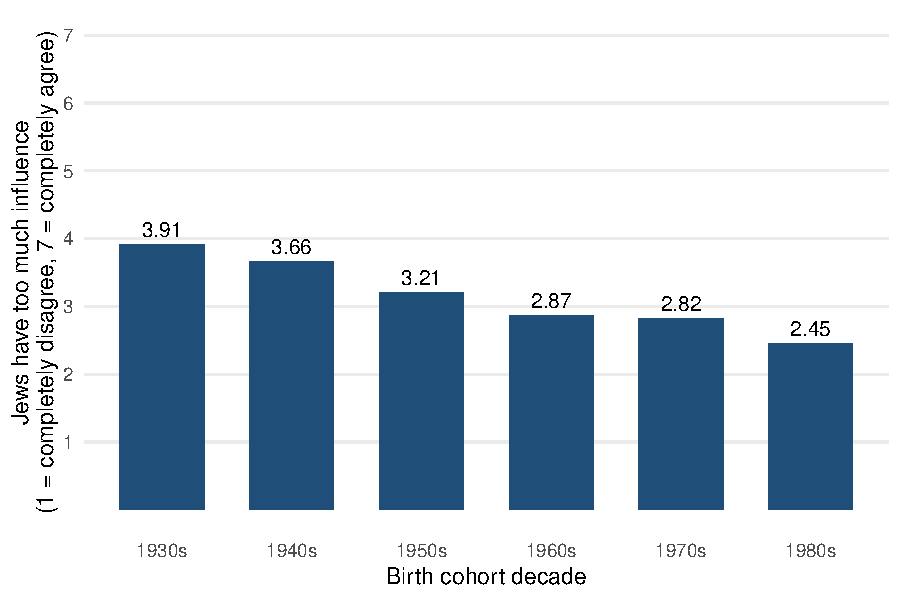
\includegraphics[width=0.8\textwidth]{figures/figure7.pdf}

  \tablenotes{Replication of Figure~7 of the paper. Mean agreement (1--7) with the statement that Jews have too much influence in the world, by decade of birth. ALLBUS 2016, respondents born in Germany 1930--1989 who are Christian or have no religion.}
\end{figure}

\subsection{Interpretation}

\instr{Appendix~B.2 shows how to read and interpret coefficients.}

\hint{Was heisst 0.16 bzw.\ 0.85 auf der 1--7-Skala? Groesse in SD (1.10 vs.\ 0.18 SD, S.\ 2364). Warum steigt der Koeffizient mit Kontrollen? Wald-Logik: 0.330 / 0.388 = 0.850.}

% Your text

% ===========================================================================
\section{Critical Evaluation}
% ===========================================================================

\subsection{Threats to internal validity}

\instr{Focus on the threat(s) to internal validity you consider most important. You can prepare this section with Worksheet~A.4 and Appendix~B.1.}

\hint{Auf 2--3 wichtigste Threats fokussieren (siehe \texttt{paper/notes.md}, Abschnitt Threats): (1) Exclusion Restriction inkl.\ Richtung der Verzerrung und Tabelle \texttt{tables/ext\_exclusion.tex}; (2) schwaches Instrument (F = 10.5, Folie 2c: F $>$ 104.7); (3) Messfehler: wenn nur Messfehler, waere $\lambda \approx 0.17$. Optional LATE.}

% Your text

\begin{teamdraft}
\par\textbf{General Threats to Identification}\par

The following threats link the concepts of the course to the paper.

\begin{itemize}
\item
  \textbf{Omitted variable bias (OLS):} ideology or a general propensity for prejudice could drive both X and Y; the authors address this with controls and Oster bounds.\footnote{(Binstok, Gould, and Kaplan 2024, p. 2350, l. 3--11; p. 2355, l. 14--19)}
\item
  \textbf{Reverse causality:} views on Israel could shape views on Jews; the authors name this threat but address it only through the IV.\footnote{(Binstok, Gould, and Kaplan 2024, p. 2355, l. 24--26)}
\item
  \textbf{Measurement error in X:} social desirability attenuates the OLS estimate towards zero; this is the authors' main explanation for IV exceeding OLS.\footnote{(Binstok, Gould, and Kaplan 2024, p. 2364, l. 27--35)}

  \begin{itemize}
  \item
    In the Twitter data, the same-day measure is noisy: the OLS coefficient rises from 0.297 (daily) to 0.561 (weekly) and 0.670 (monthly).\footnote{(Binstok, Gould, and Kaplan 2024, p. 2343, l. 8--16)}
  \end{itemize}
\item
  \textbf{Weak instrument:} a weak first stage biases 2SLS towards OLS and makes inference unreliable; this applies to the specification with linear age and to the interviewer IV.\footnote{(Binstok, Gould, and Kaplan 2024, p. 2356, l. 17--20; p. 2365, l. 4--6)}
\item
  \textbf{Invalid exclusion restriction:} the birth cohort may affect views on Israel directly, for example through war experience or post-war politics. The authors concede that this key assumption cannot be tested.\footnote{(Binstok, Gould, and Kaplan 2024, fn. 23, p. 2361, l. 41--43)}
\item
  \textbf{Local average treatment effect (LATE):} the IV identifies the effect for individuals whose antisemitism was shifted by childhood indoctrination, i.e. mainly older Germans. This is a concept from the course and is not discussed in the paper.
\item
  \textbf{Sample restriction and external validity:} the sample covers only German-born Christians and non-religious respondents, so the results apply to people without a direct link to the conflict.\footnote{(Binstok, Gould, and Kaplan 2024, p. 2333, l. 24--27)}
\item
  \textbf{Small sample for the IV:} there are too few respondents born 1930--1945 to estimate the IV within subgroups.\footnote{(Binstok, Gould, and Kaplan 2024, p. 2361, l. 20--22)}
\item
  \textbf{Standard errors:} heteroskedasticity-robust for ALLBUS and clustered by district for Twitter.\footnote{(Binstok, Gould, and Kaplan 2024, notes to Tables 7 and 10; notes to Tables 2 and 3)}
\end{itemize}


\end{teamdraft}

% Optional table for this section:
% \begin{table}[htbp]
%   \centering
%   \caption{Does the instrument shift other worldviews?}
%   \label{tab:excl}
%   \begin{tabular}{lccc}
\toprule
Dependent variable & Born 1930--45 & SE & $N$ \\
\midrule
Jews too much influence (first stage) & $0.519^{***}$ & (0.118) & 2,585 \\
Political spectrum (left-right) & $0.241^{**}$ & (0.101) & 2,694 \\
Very proud German & $0.044$ & (0.027) & 2,718 \\
No religion & $-0.067^{**}$ & (0.028) & 2,795 \\
Abitur (``college'') & $-0.038^{*}$ & (0.023) & 2,795 \\
Foreigners enrich culture & $-0.420^{***}$ & (0.109) & 2,777 \\
Islam fits in & $-0.240^{**}$ & (0.095) & 2,746 \\
Israel unjust (reduced form) & $0.337^{***}$ & (0.099) & 2,531 \\
Israeli policy justifies antisemitism (reduced form) & $0.618^{***}$ & (0.115) & 2,561 \\
\bottomrule
\end{tabular}

%   \tablenotes{OLS of each variable on an indicator for being born 1930--1945, controlling for being born before 1960 and gender (Table~9, third panel, of the paper). Robust (HC1) standard errors. *** $p<0.01$, ** $p<0.05$, * $p<0.1$.}
% \end{table}

\subsection{Overall assessment}

\instr{What do you think about the overall validity of the paper? Three or four sentences are enough.}

% Your text

% ===========================================================================
\section{Extension and Robustness}
% ===========================================================================

\subsection{Extension}

\instr{This part should include your extension. Test whether the main conclusion continues to hold when you change something the authors did not change. Discuss the extension in theory (as above briefly describe your empirical strategy and assumptions) and show us your main result.}

\hint{Zwei Teile: (A) weak-IV-robuste Inferenz (tF: p = 0.14; AR: [0.33, 2.18]) und (C) plausibly exogenous (AR-KI enthaelt 0 ab $\delta = 0.13$; IV = OLS bei $\delta = 0.27$). Staerken, Grenzen, was man verbessern koennte. Zahlen: \texttt{code/README.md}.}

% Your text

\begin{table}[htbp]
  \centering
  \caption{Weak-instrument-robust inference for the IV estimates}
  \label{tab:ext}
  \resizebox{\textwidth}{!}{\begin{tabular}{lcccccccc}
\toprule
 & (1) & (2) & (3) & (4) & (5) & (6) & (7) & (8) \\
\midrule
First stage: born 1930--45 & 0.874 & 0.507 & 0.396 & 0.388 & 0.386 & 0.371 & 0.361 & 0.353 \\
 & (0.103) & (0.120) & (0.120) & (0.120) & (0.120) & (0.121) & (0.119) & (0.119) \\
First-stage $F$ (robust) & 71.9 & 17.9 & 11.0 & 10.5 & 10.4 & 9.4 & 9.2 & 8.9 \\
Reduced form: born 1930--45 & 0.428 & 0.299 & 0.329 & 0.330 & 0.353 & 0.317 & 0.338 & 0.346 \\
 & (0.088) & (0.102) & (0.102) & (0.103) & (0.105) & (0.106) & (0.106) & (0.105) \\
\midrule
2SLS: Jews too much influence & 0.489 & 0.589 & 0.830 & 0.850 & 0.914 & 0.854 & 0.934 & 0.981 \\
 & (0.111) & (0.227) & (0.330) & (0.339) & (0.358) & (0.363) & (0.382) & (0.401) \\
95\% CI, $\pm 1.96$ & [0.27, 0.71] & [0.14, 1.03] & [0.18, 1.48] & [0.18, 1.51] & [0.21, 1.61] & [0.14, 1.57] & [0.18, 1.68] & [0.20, 1.77] \\
tF critical value & 2.04 & 2.70 & 3.28 & 3.34 & 3.37 & 3.55 & 3.60 & 3.69 \\
95\% CI, tF & [0.26, 0.71] & [-0.02, 1.20] & [-0.25, 1.91] & [-0.28, 1.98] & [-0.29, 2.12] & [-0.44, 2.15] & [-0.44, 2.31] & [-0.50, 2.46] \\
$p$-value, tF & 0.000 & 0.060 & 0.133 & 0.142 & 0.137 & 0.195 & 0.183 & 0.194 \\
95\% CI, Anderson--Rubin & [0.29, 0.74] & [0.20, 1.24] & [0.32, 2.09] & [0.33, 2.18] & [0.37, 2.35] & [0.29, 2.38] & [0.36, 2.61] & [0.39, 2.82] \\
\midrule
Observations & 2,438 & 2,438 & 2,438 & 2,438 & 2,378 & 2,330 & 2,321 & 2,309 \\
\bottomrule
\end{tabular}
}

  \tablenotes{Columns (1)--(8) correspond to Table~10 of the paper (outcome: Israel is unjust to take Palestinian land). First stage and reduced form: coefficient on the indicator for being born 1930--1945, same sample and controls as the 2SLS regression; HC0 standard errors. The tF critical value and confidence interval follow Lee, McCrary, Moreira and Porter (2022). The Anderson--Rubin (AR) confidence set is heteroskedasticity-robust and valid regardless of the strength of the instrument.}
\end{table}

\begin{figure}[htbp]
  \centering
  \caption{Sensitivity of the main IV estimate to violations of the exclusion restriction}
  \label{fig:ext}
  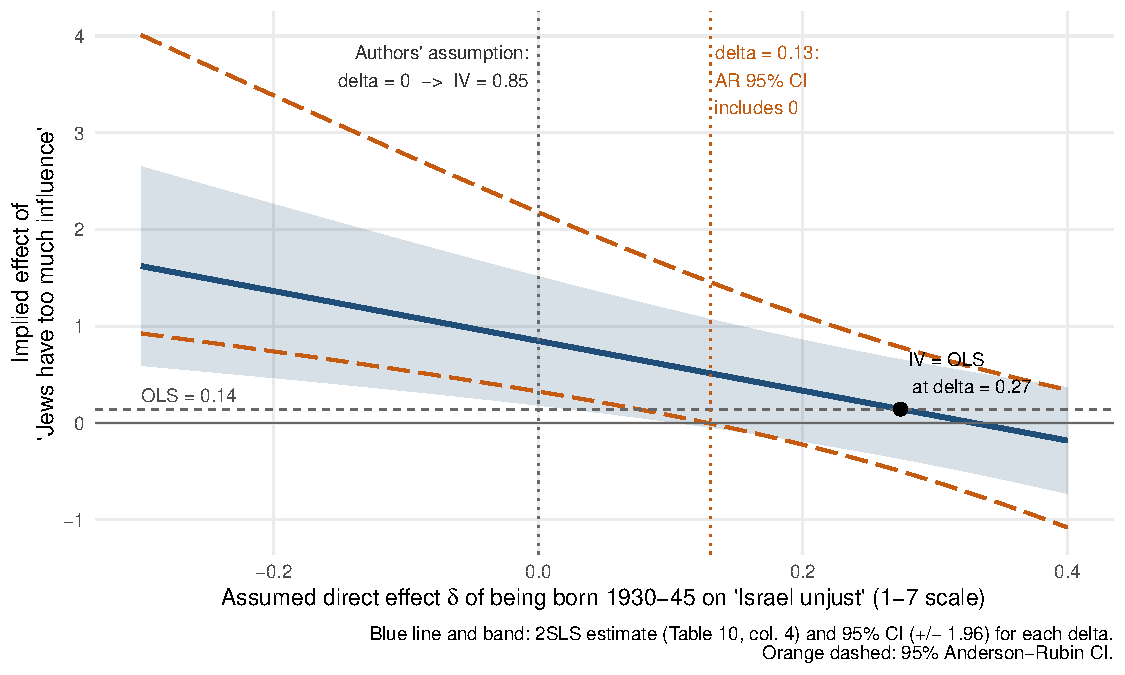
\includegraphics[width=0.9\textwidth]{figures/ext_plausexog.pdf}

  \tablenotes{Table~10, column 4. For each assumed direct effect $\delta$ of being born 1930--1945 on the outcome, the figure shows the implied 2SLS estimate $\beta(\delta) = (\text{reduced form} - \delta)/\text{first stage}$ with its conventional and Anderson--Rubin 95\% confidence intervals (Conley, Hansen and Rossi 2012). The dashed horizontal line is the comparable OLS estimate (Table~7, column 3).}
\end{figure}

% Alternative figure (all Table 10 columns, three types of CIs):
% 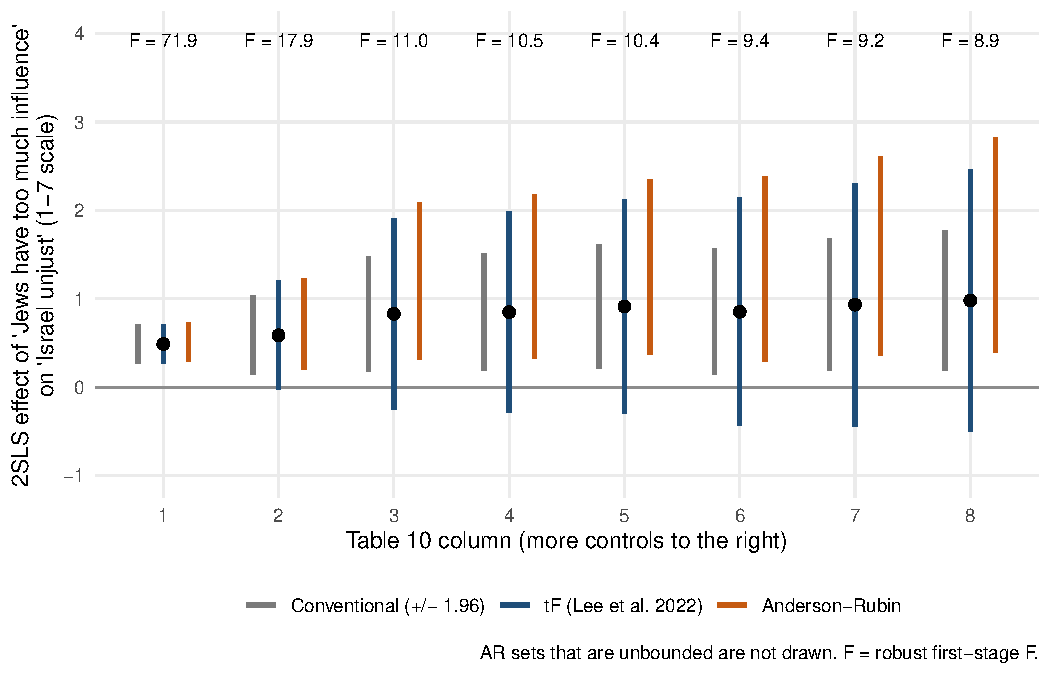
\includegraphics[width=0.9\textwidth]{figures/ext_weakiv.pdf}

\subsection{Ideal empirical strategy}

\instr{Please describe the best empirical design you could implement if there were no restrictions on data availability (or on money and ethics, in the case of an experiment).}

\hint{Noch offen -- im Team ueberlegen (Ideen in \texttt{paper/notes.md}, Extension D).}

% Your text

% ===========================================================================
\section{Conclusion}
% ===========================================================================

% Your text

% ===========================================================================
\begin{thebibliography}{9}
% ===========================================================================
\bibitem{paper} Binstok, N., Gould, E.~D., \& Kaplan, T. (2024). Policies or prejudices? An analysis of antisemitic and anti-Israel views on social media and social surveys. \textit{Journal of the European Economic Association} 22(5), 2329--2373. \url{https://doi.org/10.1093/jeea/jvae013}

\bibitem{allbus} GESIS -- Leibniz-Institut f\"ur Sozialwissenschaften (2018). German General Social Survey -- ALLBUS 2016. GESIS Data Archive, Cologne. ZA5252 Data file Version 1.0.0. \url{https://doi.org/10.4232/1.12837}

\bibitem{vv} Voigtl\"ander, N., \& Voth, H.-J. (2015). Nazi indoctrination and anti-Semitic beliefs in Germany. \textit{Proceedings of the National Academy of Sciences} 112(26), 7931--7936.

\bibitem{lmmp} Lee, D.~S., McCrary, J., Moreira, M.~J., \& Porter, J. (2022). Valid t-ratio inference for IV. \textit{American Economic Review} 112(10), 3260--3290.

\bibitem{ar} Anderson, T.~W., \& Rubin, H. (1949). Estimation of the parameters of a single equation in a complete system of stochastic equations. \textit{Annals of Mathematical Statistics} 20(1), 46--63.

\bibitem{chr} Conley, T.~G., Hansen, C.~B., \& Rossi, P.~E. (2012). Plausibly exogenous. \textit{Review of Economics and Statistics} 94(1), 260--272.

\bibitem{oster} Oster, E. (2019). Unobservable selection and coefficient stability: Theory and evidence. \textit{Journal of Business \& Economic Statistics} 37(2), 187--204.
\end{thebibliography}

% ===========================================================================
\clearpage
\appendix
\section{Replication Worksheets}
% ===========================================================================

\instr{Please fill in these worksheets and submit them together with your report. Keywords are sufficient. The worksheets do not count toward the page limit. Add rows or columns where your paper requires it.}

\hint{A.1--A.3 sind mit Fakten aus Paper und Code vorausgefuellt -- bitte pruefen. A.4 (blau) sind Vorschlaege aus unserer Besprechung: selbst bewerten und anpassen.}

\subsection{The paper at a glance}

{\renewcommand{\arraystretch}{1.4}%
\begin{tabularx}{\textwidth}{@{}>{\raggedright\arraybackslash}p{0.36\textwidth}L@{}}
\toprule
Field & Your entry \\
\midrule
Paper & Binstok, Gould \& Kaplan (2024), ``Policies or Prejudices? An Analysis of Antisemitic and Anti-Israel Views on Social Media and Social Surveys,'' \textit{JEEA} 22(5), 2329--2373. doi:10.1093/jeea/jvae013 \\
Replication package & [Link zum Replikationspaket eintragen -- derselbe wie bei praxai.ch] \\
Additional data sources & ALLBUS 2016, GESIS ZA5252 v1.0.0, doi:10.4232/1.12837 [Zugriffsdatum eintragen] \\
Outcome ($Y$) & Agreement 1--7: ``It is unjust that Israel is taking away land from the Palestinians'' (mj06) \\
Treatment or variable of interest ($X$) & Agreement 1--7: ``Jews have too much influence in the world'' (mj01) \\
Unit of observation & Individual survey respondent \\
Setting and period & Germany, ALLBUS 2016 (cross-section) \\
Comparison & Respondents born 1930--1945 (Nazi-era childhood) vs.\ 1946--1960, holding the broad cohort (before/after 1960) constant \\
Main method & OLS with stepwise controls; IV-2SLS (instrument: born 1930--1945) \\
Result replicated & Table 6 (col.\ 1), Table 7 (cols.\ 1--7), Table 9 (third panel, first stage and reduced form), Table 10 (cols.\ 1--8, both outcomes), Figure 7 \\
Software and version & R [Version eintragen, z.\,B.\ R 4.4]; packages haven, sandwich, ivreg, ggplot2 \\
Code & \url{https://github.com/tiny-dora/empirical-methods-replication} (folder \texttt{code/}) \\
\bottomrule
\end{tabularx}}

\subsection{Key variables}

{\renewcommand{\arraystretch}{1.4}%
\begin{tabularx}{\textwidth}{@{}>{\raggedright\arraybackslash}p{0.25\textwidth}
  >{\raggedright\arraybackslash}p{0.25\textwidth}
  >{\raggedright\arraybackslash}p{0.16\textwidth}
  L@{}}
\toprule
Role & Name in paper & Name in dataset & Definition and unit \\
\midrule
Outcome ($Y$) & Israel---unjust to take Palestinian land & mj06 & Agreement scale 1 (completely disagree) to 7 (completely agree) \\
Variable of interest ($X$) & Jews---too much influence & mj01 & Agreement scale 1--7; higher = more antisemitic \\
Instrument ($Z$), if IV & Cohort: born 1930--1945 & yborn & Dummy = 1 if born 1930--1945 \\
Main controls ($W$) & Gender, born before 1960, education, county \% foreigners and unemployment, state, political spectrum, religion, very proud German, foreigners enrich culture, Islam fits in & sex, yborn, educ, gr01, gr03, land, pa01, rd01, pn11, mp03, mm02 & Dummies; education, state, political spectrum, religion as categories; county variables as bracket codes (linear); attitudes 1--7 \\
\bottomrule
\end{tabularx}}

\medskip\noindent
Sample: 2,336 observations (Table~6; regressions 2,309--2,585 depending on missing values), individuals born in Germany 1930--1990, Christian or no religion; one cross-section (2016).

\subsection{Reconciling differences}

Importantly, here you do not have to check everything. In the main text, please explain where you believe the difference between your results is coming from based on the suggestions.

{\renewcommand{\arraystretch}{1.4}%
\begin{tabularx}{\textwidth}{@{}>{\raggedright\arraybackslash}p{0.45\textwidth}L>{\raggedright\arraybackslash}p{0.15\textwidth}@{}}
\toprule
Possible source & What we checked & Effect on $\beta$ \\
\midrule
Data version & Same file as authors (ZA5252 v1.0.0) & none \\
Sample restrictions and missing values & Same restrictions as do-file; Stata treats missing in \texttt{gen x = (cond)} as 0 and missing \texttt{non\_christian} as ``not 1'' -- replicated in R & none (N identical) \\
Construction of variables (definitions, deflators, logs of zero) & Reverse coding of two items; first factor = Stata principal factor (not \texttt{factanal}); ``college'' = Abitur; ``native'' = citizen since birth & none \\
Sample weights & None (as authors) & none \\
Fixed effects and dropped singletons & State dummies; no singletons issue & none \\
Standard errors (clustering, small-sample corrections) & OLS \texttt{reg, robust} = HC1; IV \texttt{ivreg2, robust} = HC0 & SE identical only with these choices \\
Software defaults (Stata, R, Python) & Factor variables and missing-value handling matched to Stata & none \\
Other (specify) & Note to Table~11 lists age controls that are not in the code (Table~10 col.\ 4 has none) & none \\
\bottomrule
\end{tabularx}}

\subsection{Threats to internal validity}

Importantly, also here you do not have to check everything but what you consider to be most important.

{\renewcommand{\arraystretch}{1.4}%
\begin{tabularx}{\textwidth}{@{}>{\raggedright\arraybackslash}p{0.18\textwidth}
  L
  >{\raggedright\arraybackslash}p{0.13\textwidth}
  L
  >{\raggedright\arraybackslash}p{0.14\textwidth}@{}}
\toprule
Threat & Potential mechanism in this paper & Direction of bias & Addressed by the authors & Convincing? \\
\midrule
Omitted variable(s) & \suggest{Ideology, general prejudice against out-groups drive X and Y (OLS)} & \suggest{likely upward (OLS)} & \suggest{Stepwise controls; coefficient rises; Oster bounds; IV} & \suggest{[selbst bewerten]} \\
Reverse causality & \suggest{Anger about Israeli policy raises antisemitic views (Y $\to$ X)} & \suggest{upward (OLS)} & \suggest{Only via IV} & \suggest{[selbst bewerten]} \\
Measurement error & \suggest{Respondents under-report antisemitism (social desirability)} & \suggest{toward zero (OLS)} & \suggest{IV; interviewer-age evidence} & \suggest{[selbst bewerten; $\lambda \approx 0.17$ needed]} \\
Sample selection & \suggest{Only native Christians/non-religious; only 2016} & \suggest{external validity} & \suggest{Stated explicitly} & \suggest{[selbst bewerten]} \\
Other (specify) & \suggest{IV: exclusion restriction (cohort affects views on Israel directly, e.g.\ war, guilt/reparations, politics); weak instrument (F = 10.5)} & \suggest{$\delta>0$: up; $\delta<0$: down; weak IV amplifies by 1/0.388} & \suggest{Controls for worldviews; broad cohort dummy insignificant; F not reported} & \suggest{[selbst bewerten]} \\
\bottomrule
\end{tabularx}}

\subsection{Reproducibility checklist}

\begin{itemize}[label=$\boxtimes$, leftmargin=*, itemsep=2pt]
  \item A README file describes the folder structure, the software and package versions, and the order in which the scripts are run. (\texttt{README.md}, \texttt{code/README.md})
  \item One master script runs the whole analysis, starting from the raw data. (\texttt{code/00\_run\_all.R})
  \item The raw data are not modified; all cleaning is done in code. (\texttt{code/01\_clean\_allbus.R})
  \item The code only uses relative file paths. (RStudio project file)
  \item Every table and figure in the report is produced by a script. (\texttt{code/02\_tables.R}, \texttt{code/03\_extension.R})
  \item Random seeds are set wherever results depend on simulation or bootstrapping. (No simulation or bootstrapping used.)
\end{itemize}

\textit{Use of AI tools (optional).} [Two or three sentences on how you used AI tools.]

\hint{Ehrlich angeben, wofuer ihr AI genutzt habt, z.\,B.\ Code-Review und Umsetzung der Extension in R, Erklaerungen von Methoden, Grammatik. Selbst formulieren.}

% ===========================================================================
\clearpage
\section{Notes on Methods}
% ===========================================================================

\instr{Delete this appendix before submitting.}

\subsection{Guide to evaluate identification methods}

\paragraph{Step 1: What is the model?}
Write the authors' main specification in one of the forms we used in class:
\begin{align*}
  \text{OLS:} \quad & y_i = x_i'\beta + \varepsilon_i = \beta_1 + \beta_2 x_{i2} + \dots + \beta_K x_{iK} + \varepsilon_i . \\
  \text{Panel data:} \quad & y_{it} = x_{it}'\beta + \alpha_i + d_t + \varepsilon_{it} \\
  \text{IV:} \quad & y_i = x_{1i}'\beta_1 + x_{2i}'\beta_2 + \varepsilon_i,
     \quad \text{with instruments } z_i' = [z_{1i}' \;\; x_{2i}']
\end{align*}
Which variable $x_{ik}$ is the variable of interest? Which variables are controls? If you use panel methods, what exactly is in $\alpha_i$ and $d_t$ in your paper? For IV, which variables are in $x_{1i}$ and which in $z_{1i}$?

\paragraph{Step 2: Which comparison identifies $\beta$?}
What do the authors compare to identify $\beta$. Is it a comparison across units, within the same unit over time, or between units that are affected differently by an instrument? Once $\alpha_i$ and $d_t$ are taken out, or once only the variation in $x_{1i}$ that comes from $z_{1i}$ is used, what variation is left?

\paragraph{Step 3: Which assumption allows a causal interpretation of $\hat{\beta}$?}
Think about the material covered in class. Which of the main assumptions have to be fulfilled to allow for a causal interpretation. For OLS we made five assumptions: linearity, mean-zero error, homoskedasticity, no serial correlation, and normal errors. Both panel data methods and IV make some additional assumptions or replace some of the assumptions with their own version. For panel data methods, we have seen that the estimators differ in what they assume about $Cov(x_{is}, \varepsilon_{it})$ and $Cov(x_{it}, \alpha_i)$. What does the estimator in your paper need? For IV, we discussed exogeneity and relevance. What do they imply and how do the authors make sure that they are fulfilled?

\paragraph{Step 4: Is the assumption plausible?}
This should be the core of your evaluation of the paper. Some questions to guide you:
\begin{itemize}[leftmargin=*, itemsep=2pt]
  \item In general: We discussed three threats to the internal validity of OLS. Ask yourself: Could $y_i$ also affect the variable of interest? Is there a third variable that drives both? Is the variable of interest measured with error?
  \item In panel data: Which of these problems can fixed effects account for and which not? Could the outcome in one  period affect the explanatory variables in a later period?
  \item For IV: Why should the instrument move $x_{1i}$? Can you think of any channel through which it might affect $y_i$ directly, or be related to something in $\varepsilon_i$?
\end{itemize}

\paragraph{Step 5: What evidence do the authors provide?}
Which tests, robustness checks or figures do the authors use to support the assumption from Steps 3 and 4? For IV, what does the first stage show, and how large is the $F$-statistic? Does the evidence provided by the authors address the concerns you raised in Step~4, or does it test something else?

\paragraph{Step 6: How are standard errors computed?}
Recall what happens when (A3) or (A4) fails. Which standard errors do the authors report? Do they cluster? If so, at which level? Are the errors potentially correlated within these clusters?

\subsection{Interpreting coefficients}

\begin{tabularx}{\textwidth}{@{}P{0.3\textwidth}L@{}}
\toprule
\textbf{Specification} & \textbf{Interpretation of $\beta_k$} \\
\midrule
$y_i$ on $x_{ik}$ & A one-unit increase in $x_{ik}$ changes $y_i$ by $\beta_k$ units. \\
$\log y_i$ on $x_{ik}$ & A one-unit increase in $x_{ik}$ changes $y_i$ by about $100\beta_k$ percent (exactly $100(e^{\beta_k}-1)$ percent). \\
$y_i$ on $\log x_{ik}$ & A one percent increase in $x_{ik}$ changes $y_i$ by about $\beta_k/100$ units. \\
$\log y_i$ on $\log x_{ik}$ & A one percent increase in $x_{ik}$ changes $y_i$ by about $\beta_k$ percent (an elasticity). \\
Binary $y_i$ (linear probability model) & A one-unit increase in $x_{ik}$ changes the probability that $y_i = 1$ by $100\beta_k$ percentage points. \\
\bottomrule
\end{tabularx}

In each case, the other explanatory variables are held constant.

\subsection{Direction of omitted variable bias}

As in class, suppose the true model is $y_i = x_i'\beta + \gamma w_i + \varepsilon_i$, but you estimate $y_i = x_i'\beta + \varepsilon_i$ and omit $w_i$. Then
\[
  E(\hat\beta_k) = \beta_k + \gamma \, \hat\beta_{w\_on\_x,k} ,
\]
where $\gamma$ is the effect of $w_i$ on $y_i$ and $\hat\beta_{w\_on\_x,k}$ is the coefficient on $x_{ik}$ in a regression of $w_i$ on $x_i$. In panel data, $\alpha_i$ plays the role of $w_i$ when it is ignored.

\begin{center}
\begin{tabular}{@{}lcc@{}}
\toprule
 & \textbf{$w_i$ raises $y_i$ ($\gamma > 0$)} & \textbf{$w_i$ lowers $y_i$ ($\gamma < 0$)} \\
\midrule
$w_i$ positively correlated with $x_{ik}$ & Upward bias & Downward bias \\
$w_i$ negatively correlated with $x_{ik}$ & Downward bias & Upward bias \\
\bottomrule
\end{tabular}
\end{center}

Upward bias makes the estimate more positive. For a negative $\beta_k$, it therefore pulls the estimate toward zero, so always say whether the bias moves the estimate toward or away from zero.

\end{document}
